\documentclass[11pt, a4paper]{article}
\usepackage[utf8]{inputenc}
\usepackage{helvet} %Fikser skrifttype
\usepackage{amsmath}
\usepackage{caption}
\usepackage{graphicx}
\usepackage{float}
\usepackage{bm}

\title{Boat lab assignment report}
\author{Gruppe 33\\ \\Edda Solem - 768666\\Nicholas Fraser Ødegård - 768620\\ Arild Stenset - 768662 }
\date{October 2017}

\begin{document}

\maketitle

\newpage
\tableofcontents
\thispagestyle{empty} % Avoid page numbering on the table of contents.

\newpage
\setcounter{page}{1}

\include{introduction}
\section{Model of the system}

The model which will be used can be stated as:

\begin{subequations}
\begin{align}
    \dot{\xi}_w &= \psi_w \label{eq: dotxi} \\
    \dot{\psi}_w &= -\omega^2_0\xi_w-2\lambda\omega_0\psi_w+K_ww_w \label{eq: dotpsi_w} \\
    \dot{\psi} &= r \label{eq: dotpsi} \\
    \dot{r} &= \frac{-1}{T}r+\frac{K}{T}(\delta-b) \label{eq: dotr} \\
    \dot{b} &= w_b \label{eq: dotb} \\
    y &= \psi+\psi_w+v \label{eq: y}
\end{align}
\end{subequations}
\section{Part 1 - Identification of the boat parameters}

\subsection{Task A}

To calculate the transfer function from $\delta$ to $\psi$, some assumptions have been taken. There are no disturbances, which means that $b = 0$. There are also no initial average heading, so $\psi(0) = 0$. \newline
By substituting (\ref{eq: dotpsi}) into (\ref{eq: dotr}) the following can be derived:


\begin{align}
    \ddot{\psi} = \frac{-1}{T}\dot{\psi}+\frac{K}{T}\delta  \nonumber    \\
    \mathcal{L}\{\ddot{\psi}\} \Rightarrow s^2\psi(s)+s\psi(0)+\psi(0) = \frac{-s}{T}\psi(s)+\psi(0)+\frac{K}{T}\delta   \nonumber   \\
    \psi(s)(s^2+\frac{s}{T}) = \frac{K}{T}\delta    \nonumber   \\
    H(s) = H_{ship}(s) = \frac{\psi}{\delta}(s) = \frac{K}{s(Ts+1)} \label{eq: deltaToPsi}
\end{align}


\subsection{Task B}
In order to determine K and T, the amplitude from the corresponding compass angle had to be found by calculation from the plots.
$A_1$ corresponds to the amplitude of the transfer function with frequency $\omega_1 = 0.005$ from Figure(\ref{fig: 1b_w0005}) and $A_2$ to frequency $\omega_2 = 0.05$ from Figure(\ref{fig: 1b_w005}).
\\
Calculated amplitudes:
\begin{equation}
    \begin{align}
        A_1 = \frac{63.34 - 4.64}{2} = 29.35 \quad \quad
        A_2 = \frac{4.23 - 2.57}{2} = 0.83 \nonumber
    \end{align}
\end{equation}

\begin{equations}
    \begin{align}
        H(j\omega_1) = \frac{K}{j\omega_1(Tj\omega_1 + 1)} \qquad A_1 = |H(j\omega_1)| = \frac{K}{\omega_1\sqrt{T^2\omega_1^2 + 1}} \nonumber
    \end{align}
\end{equations}

\begin{equation}
    \begin{align}
        K^2 = A_1^2\omega_1^2(T^2\omega_1^2 + 1) \label{eq: K_2_1}
    \end{align}
\end{equation}

\begin{equations}
    \begin{align}
        H(j\omega_2) = \frac{K}{j\omega_2(Tj\omega_2 + 1)} \qquad A_2 = |H(j\omega_2)| = \frac{K}{\omega_2\sqrt{T^2\omega_2^2 + 1}} \nonumber
    \end{align}
\end{equations}
\begin{equation}
    \begin{align}
        K^2 = A_2^2\omega_2^2(T^2\omega_2^2 + 1) \label{eq: K_2_2}
    \end{align}
\end{equation}
\\
By setting equation (\ref{eq: K_2_1}) equal to (\ref{eq: K_2_2}) and inserting $A_1$, $A_2$, $\omega_1$ and $\omega_2$ we get:
\begin{equation}
    \begin{align}
        T = \sqrt{\frac{A_1^2\omega_1^2 - A_2^2\omega_2^2}{A_2^2\omega_2^4 - A_1^2\omega_1^4}} = 72.52 \quad and \quad K = 0.156  \label{eq: T}
        \end{align}
\end{equation}
\newpage
The model is now given by:
\begin{equation}
    \begin{align}
        H(s) = \frac{\psi}{\delta}(s) = \frac{0.156}{72.52s^2+s}
    \end{align}
\end{equation}
\\

\subsection{Task C}
When trying to do the same as task B only with waves and measurement noise on, we noticed that for $\omega_1$, it is possible to get a good estimate of the paramteres K and T, which clearly can be seen i Figure(\ref{fig: 1c_w0005}). For the second frequency $\omega_2$ the case is very different, the signal is very noisy and hard to get something useful out of, this signal is found in Figure(\ref{fig: 1c_w005}).
\\

\subsection{Task D}
By adding a $1^{\circ}$ step response to the rudder and comparing the model from the transfer function with the real ship-response, it is noticeable that the approximation is good the first 500 seconds. After this the difference between the two responses is increasing with time, which can be found in Figure(\ref{fig: 1d_compare}).
\newpage


\section{Task 2 - Identification of wave spectrum model}
\section{Task 3 - Control system design}
\section{Task 4 - Observability}
\section{Part 5 - Discrete Kalman filter}
\section{Appendix A - Part 1}

\begin{figure}[H]
    \centering
    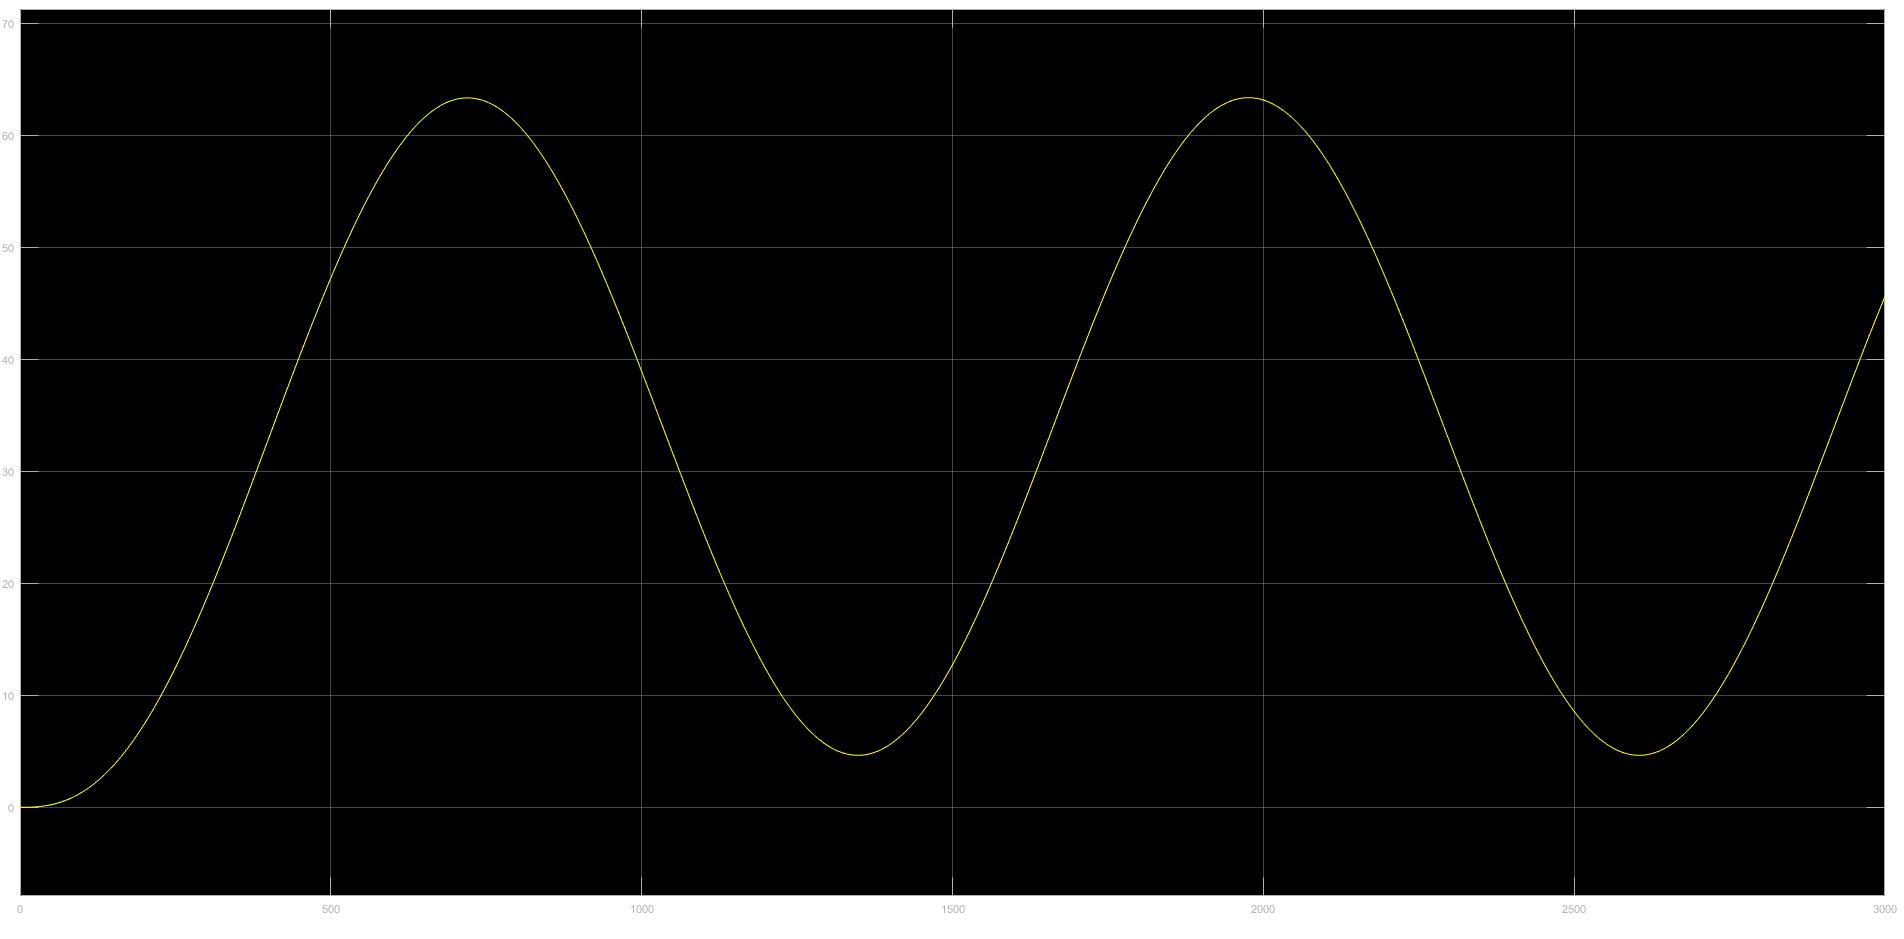
\includegraphics[width=1\textwidth]{Plots/1b_w0005.jpg}
    \caption{Plot of the compass with a sine wave set to $w1 = 0.005$ and $A=1$}
    \label{fig: 1b_w0005}
\end{figure}

\begin{figure}[H]
    \centering
    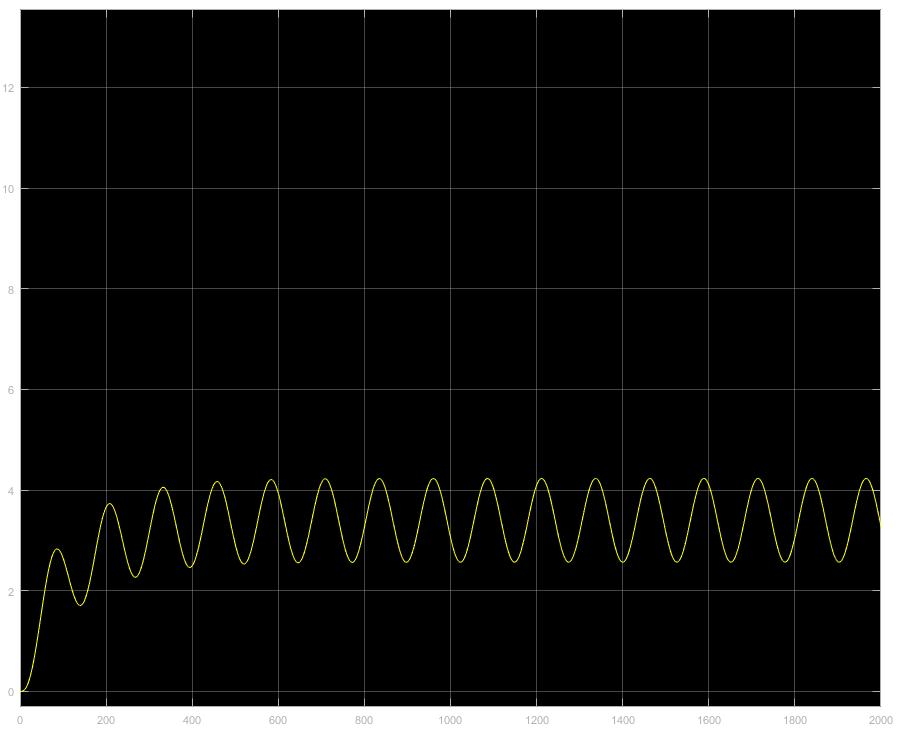
\includegraphics[width=1\textwidth]{Plots/1b_w005.jpg}
    \caption{Plot of the compass with a sine wave set to $w1 = 0.05$ and $A=1$}
    \label{fig: 1b_w005}
\end{figure}

\begin{figure}[H]
    \centering
    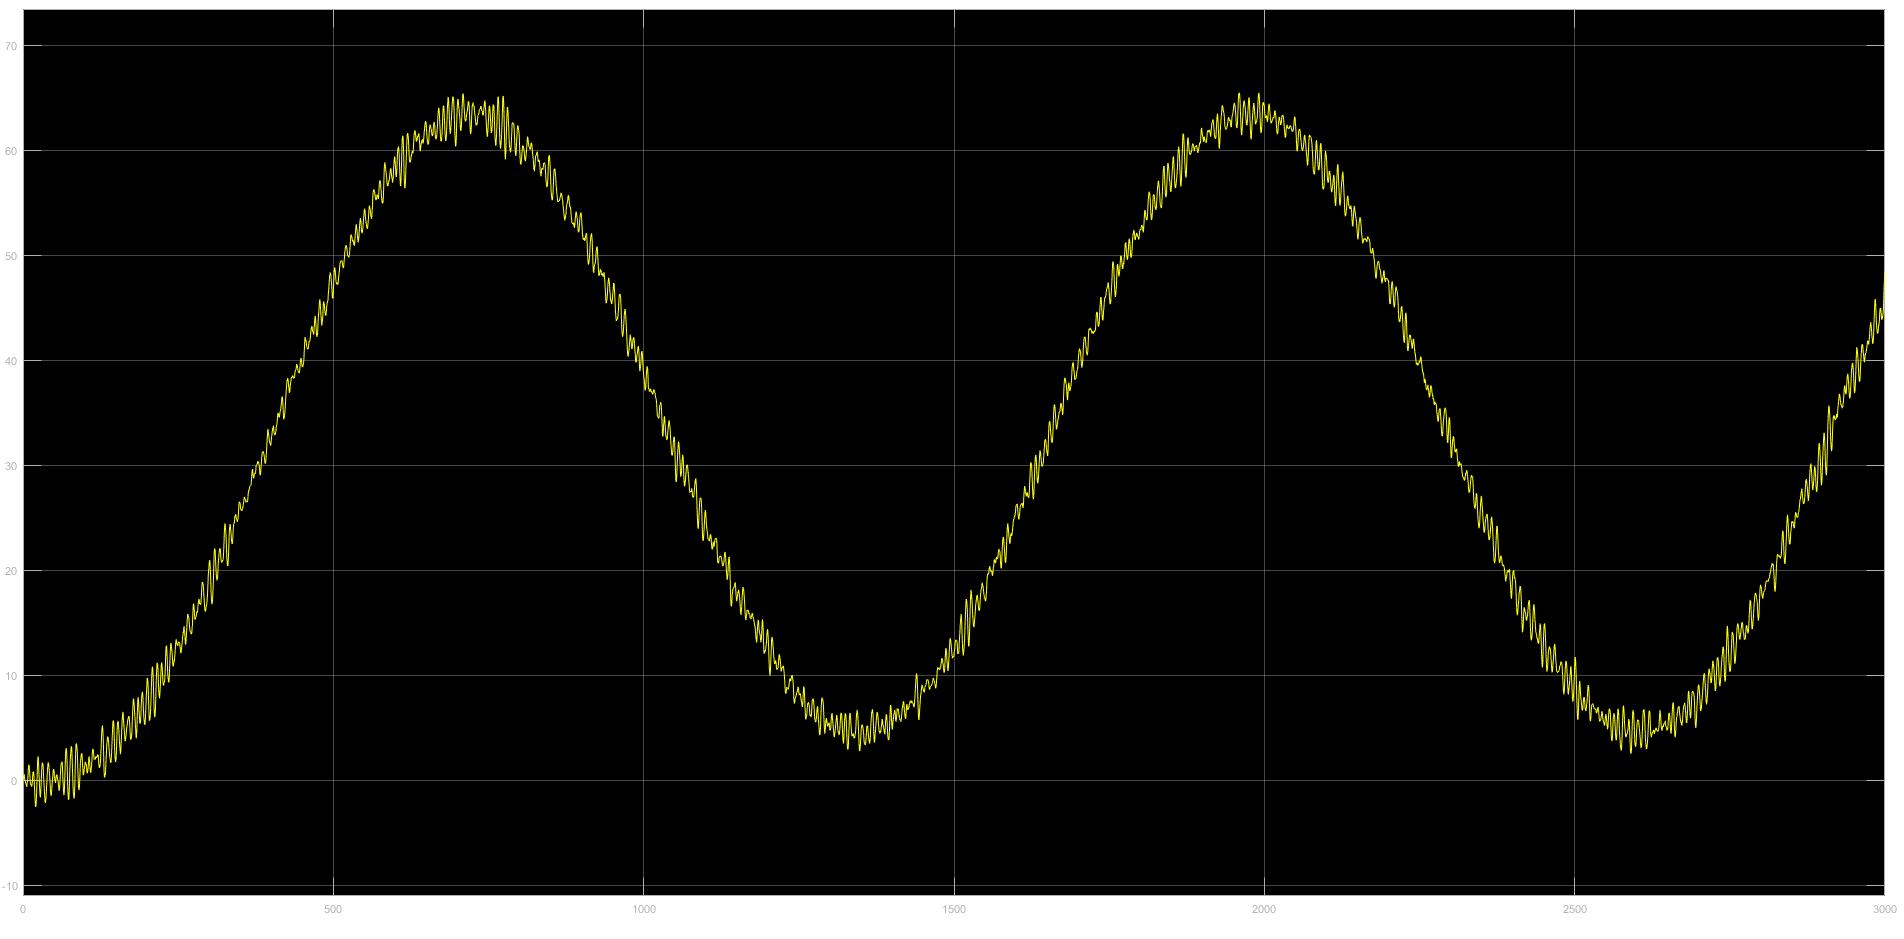
\includegraphics[width=1\textwidth]{Plots/1c_w0005.jpg}
    \caption{Plot of the compass with a sine wave set to $w1 = 0.05$ and $A=1$, in addition to measurement noise and waves}
    \label{fig: 1c_w0005}
\end{figure}

\begin{figure}[H]
    \centering
    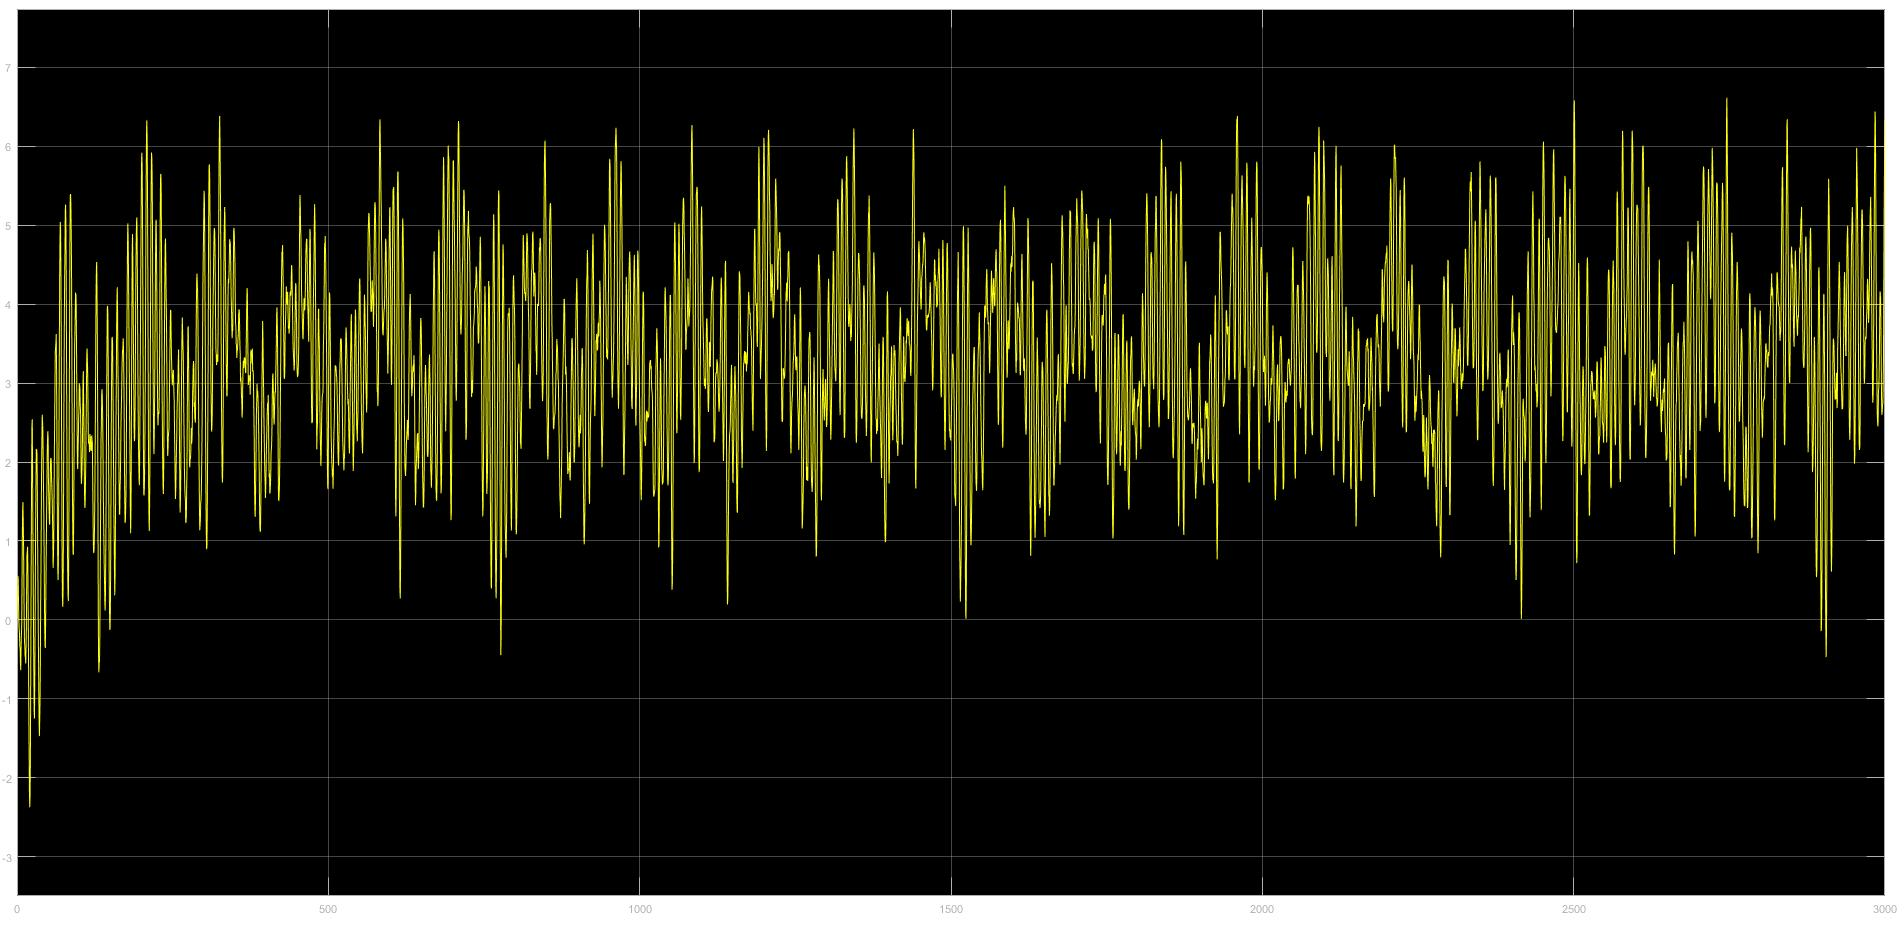
\includegraphics[width=1\textwidth]{Plots/1c_w005.jpg}
    \caption{Plot of the compass with a sine wave set to $w1 = 0.05$ and $A=1$, in addition to measurement noise and waves}
    \label{fig: 1c_w005}
\end{figure}

\begin{figure}[H]
    \centering
    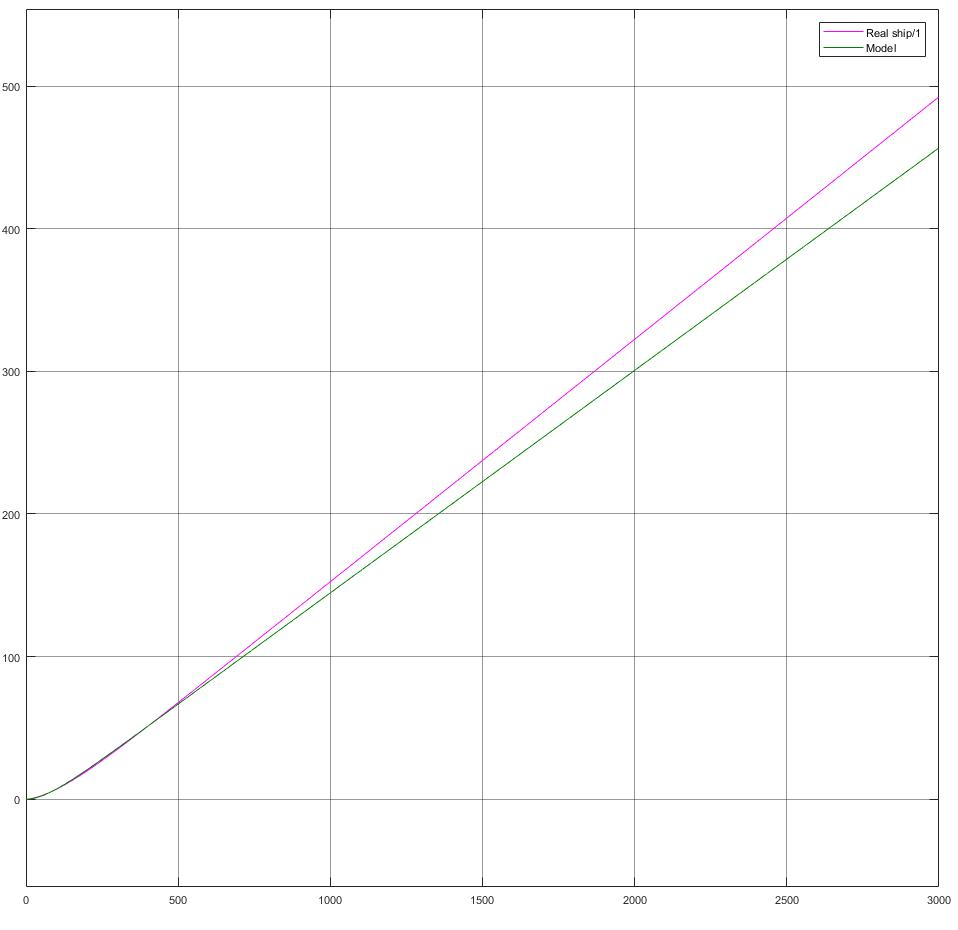
\includegraphics[width=1\textwidth]{Plots/1d_compare.jpg}
    \caption{Plot of the compass with FYLL INN NOE TEKSTVAAS}
    \label{fig: 1d_compare}
\end{figure}

\newpage
\nocite{*}
\bibliographystyle{unsrt} %Fikser silen til biblioteket sånn at ingenting går til helvete
\addcontentsline{toc}{section}{References} %Legger til kildeliste i table of content
\bibliography{kilder} %Printer referanser

\end{document}
